
\marginpar{\href{https://youtu.be/3MOahpLxj6A}{Video}} Reading: 2.1-2.3 start 2.4

\begin{figure}[h]
\centering
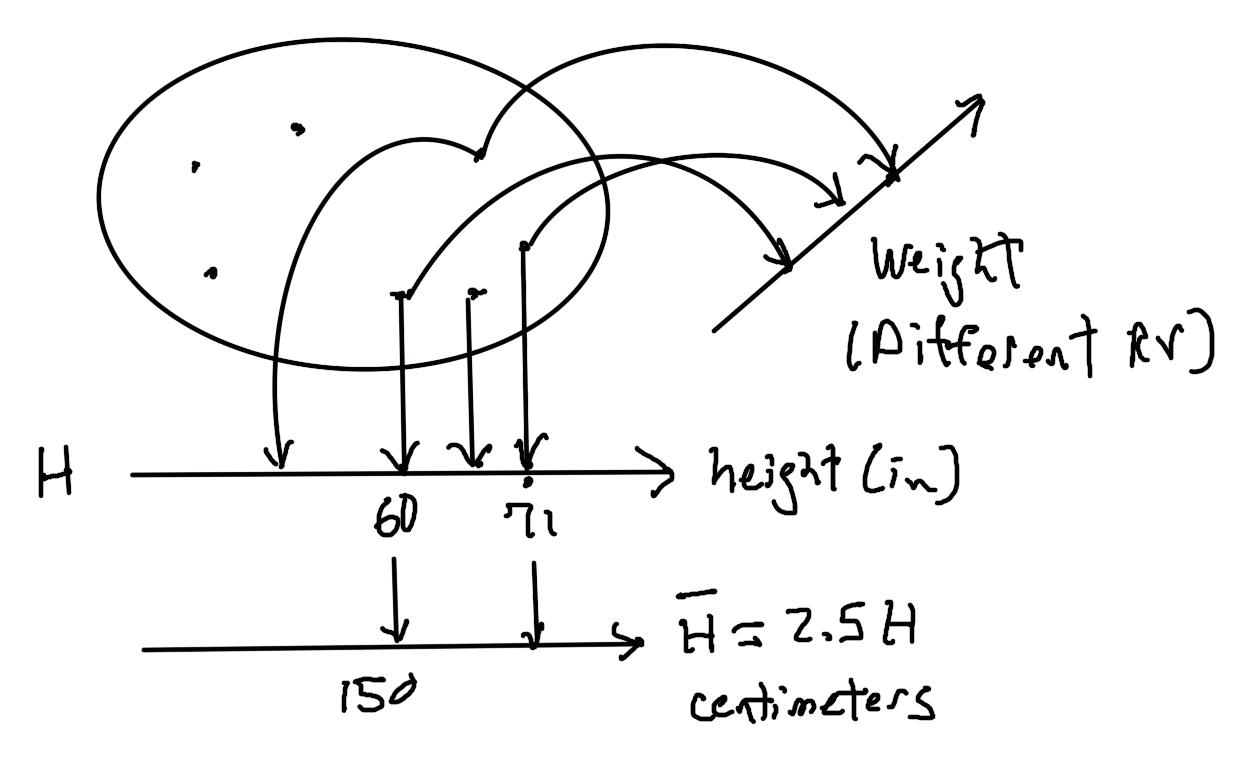
\includegraphics[width=5cm, height=4cm]{images/L05/diff_rvs.jpeg}
\caption{Experiment with Several RVs}
\end{figure}

\marginpar{(9:25)} Notation
\begin{itemize}
    \item Random variable X - function $\Omega \rightarrow \mathbb{R}$
    \item numerical value x - the amount of output of the function ($\in \mathbb{R})$
\end{itemize}

\subsection{PMF}

\marginpar{(11m)}

\begin{figure}[h]
\centering
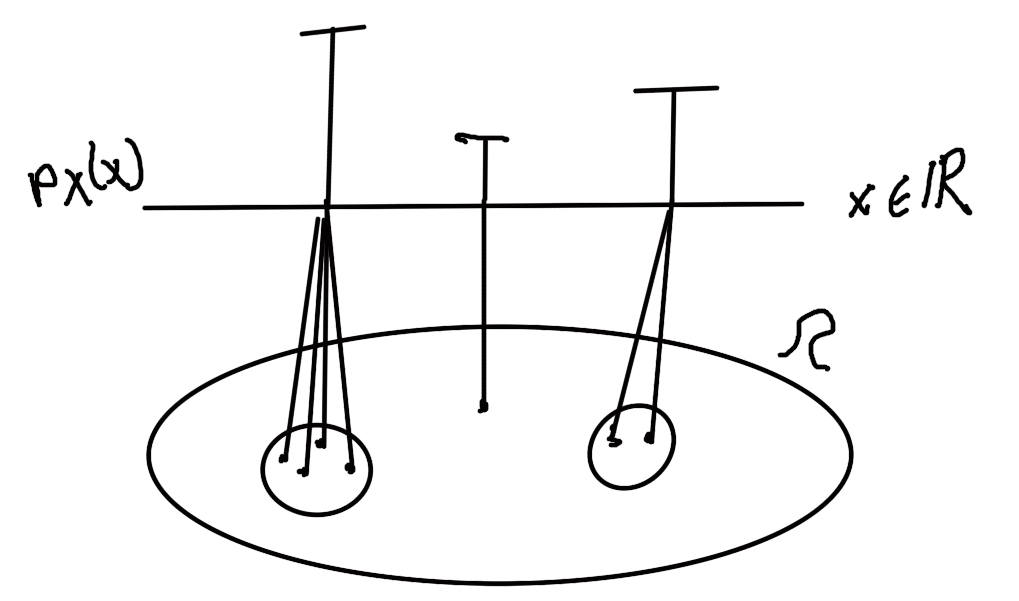
\includegraphics[width=5cm, height=4cm]{images/L05/pmf_px.jpeg}
\caption{Different RVs}
\end{figure}

\subsection{Example: \# tosses until get H (geometric RV)}

\begin{align*}
    p_X(x)=P(X=x)=P({\omega \in \Omega s.t. X(\omega)=x})
\end{align*}

\marginpar{(14:40)}

$$(1-p)^{k-1}p$$

```

\edef\mylst{"p","p(1-p)"}

\marginpar{(17m)}
\begin{figure}[h]
\centering
% 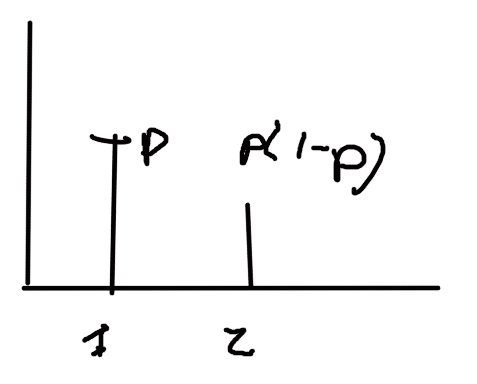
\includegraphics[width=5cm, height=4cm]{images/L05/geometric.jpeg}
\begin{tikzpicture}[scale = 0.7]
\begin{axis} [ymin = 0, ymax = 0.75, xmin = 0, xmax = 2.5,
        y tick label style={
        /pgf/number format/.cd,
            fixed,
            precision=2,
        /tikz/.cd,
        nodes near coords=\pgfmathsetmacro{\mystring}{{\mylst}[\coordindex]}\mystring,
    }]
\addplot+[ycomb] plot coordinates { (1, .5) (2, .3)}; 
\end{axis}
\end{tikzpicture}

\caption{Geometric PMF}
\end{figure}

\subsection{Example: Two independent rolls of fair tetrahedral die}

\marginpar{(18:50)}

\begin{figure}[h]
\centering
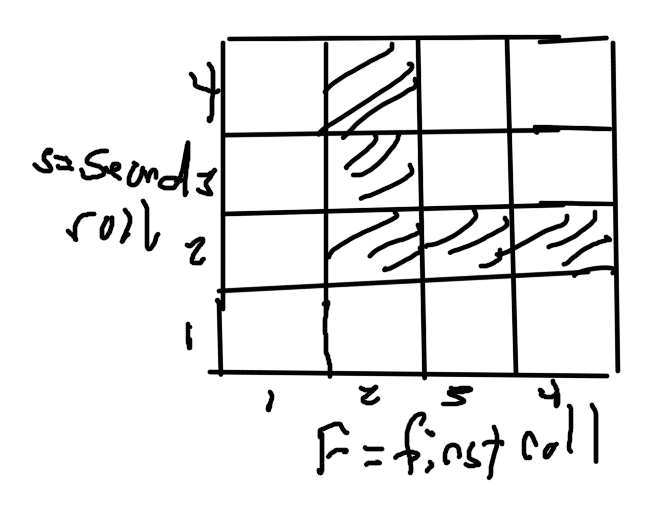
\includegraphics[width=5cm, height=4cm]{images/L05/min_2die_roll.jpeg}
\caption{Sample Space}
\end{figure}

\begin{itemize}
    \item F: outcome of first throw 2
    \item S: outcome of second throw 3
    \item X=min(F,S)
\end{itemize}

PMF: 
\begin{align*}
p_X(x)=5\frac{1}{16}=\frac{5}{16}
\end{align*}

\subsection{Binomial PMF}

\marginpar{(21m)}

X: number of heads in n fixed independent coin tosses

$P(H)=p$, let n=4

There are 6 events:
\begin{align*}
p_X(2)=P(HHTT) + P(HTHT) + \cdots + P(TTHH)\\
=6p^2(1-p)^2 \\
={4 \choose 2} p^2(1-p)^2 \\
\end{align*}

In general:

\begin{align}
p_X(k)={n \choose k} p^k(1-p)n-k, \qquad k=0,\ldots,n
\end{align}
\myequations{Binomial PMF}

% \begin{align*}
% p_X(k)=\binom{n}{k} p^k(1-p)n-k, \qquad k=0,\ldots,n\\
% \end{align*}


\marginpar{(23:25)}
\begin{figure}[h]
\centering
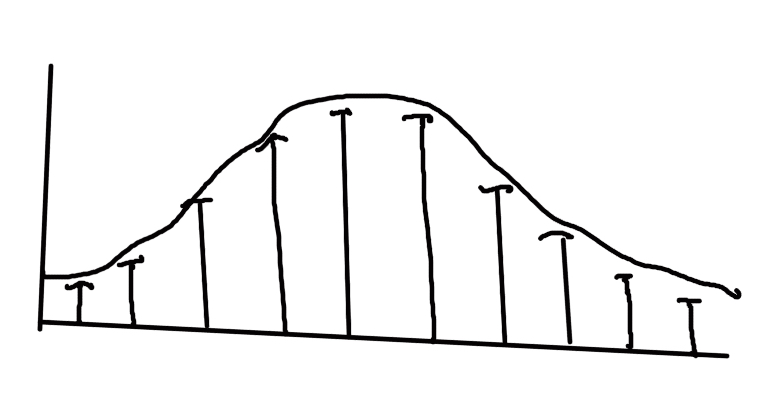
\includegraphics[width=5cm, height=4cm]{images/L05/bern_norm_approx.jpeg}
\caption{Large n gives bell curve}
\end{figure}

\subsection{Expected Value of a Random Variable}

\marginpar{(25:15)}

\begin{figure}[h]
\centering
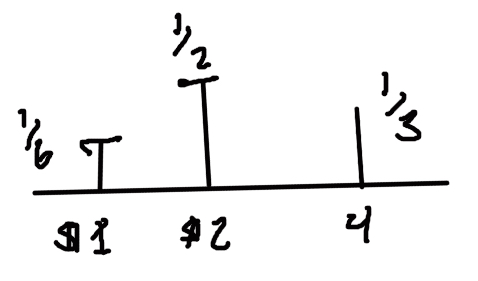
\includegraphics[width=5cm, height=4cm]{images/L05/EX_rv.jpeg}
\caption{PMF Payout}
\end{figure}

\begin{align*}
\frac{1}{6}\cdot 1 + \frac{1}{2}2 + \frac{1}{3}4 = 2.5, \qquad \text{avg payout}
\end{align*}

Expected value:
\begin{align*}
\sum_x p_X(x) \cdot x
\end{align*}
Note, this is also the center of gravity.

\subsection{Properties of Expectation}

\marginpar{(30:45)}

\begin{figure}[h]
\centering
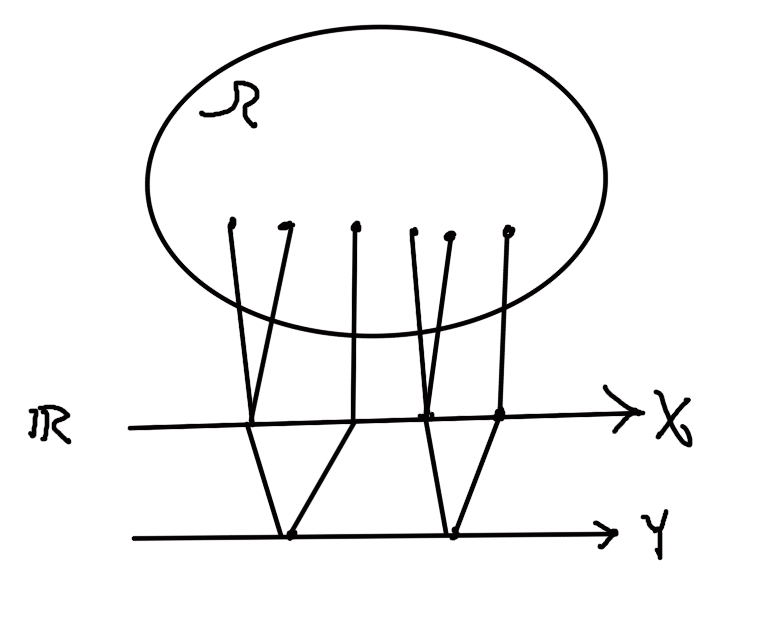
\includegraphics[width=5cm, height=4cm]{images/L05/EX_properties.jpeg}
\caption{Properties}
\end{figure}

\marginpar{(42:45)} In general, cannot reason on the average.  Only if $g(X)$ is linear.


\subsubsection{Properties}
$\alpha, \beta$ are constants

\begin{align}
&E(\alpha] = \alpha\\
&E(\alpha X] = \alpha E[X]\\
&E[\alpha X + \beta] = \alpha E[X] + \beta
\end{align}
\myequations{Properties of Expectation}

\textbf{Proof: $E[\alpha X]= \alpha E[X]$}

MISSING

\subsection{Variance Properties}

\marginpar{(43m)}

\begin{align}
var(\alpha X + \beta) = \alpha^2 var(X)
\end{align}
\myequations{Properties of Variance}

Adding a constant has no affect to expectation.